\section{Introduction}
\label{sec:intro}

\begin{figure*}
    \center
    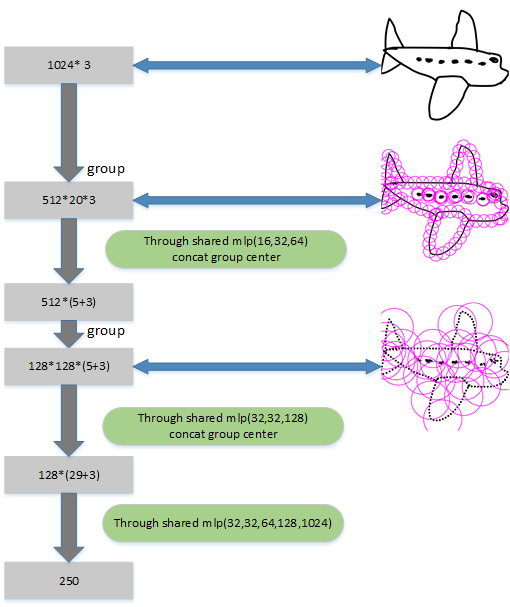
\includegraphics[width=7in]{images/sketchpointnet.png}
    \fcaption{SketchPointNet architecture.}
    \label{fig:sketchpointnet}
\end{figure*}

With the popularity of mobile and potable devices, sketching is getting easier for common users. As a powerful and effective tool for communication, freehand sketches have drawn a large amount of attentions in image processing research. 
Many approaches have bee proposed for sketch recognition~\cite{Eitz2012HowDH, LiHSG15, Schneider2014SketchCA, Yu2015SketchaNetTB, Seddati2015DeepSketchDC, Dupont2016DeepSketch2D}. 


%%%  Characteristic of freehand sketch
While been drawn on 2D devices, freehand sketches can be naturally considered as a special types of digital images.
However, their unique characteristics make sketch recognition greatly different from natural image classification. 
%
Firstly, freahand sketches for the same object vary significantly among different users. 
Sketch is a very brief representation without any color or texture details. 
%
While shape is the only hint that can be extracted from sketches, sketch recognition severely suffers from shape distortions, which vary drastically from non-experts users to professional artists. 
Moreover, the level of details presents a wide range, which makes the sketch recognition significantly challenging.
%
Secondly, sketches are much \emph{sparser} than natural images. 
From the perspective of pixel array, a large portion of pixels in a sketch image are blank. 
% Images contains richer information such as texture and dilation. 
Thirdly, the stroke pattern is also carried in the order of the strokes been drawing in a sketch. As claimed in previous research~\cite{Eitz2012HowDH}, sketches are typically drawn in a coarse-to-fine strategy. Details are usually added to the sketch later with short strokes. 
Therefore, designing a technique for sketch classification should take the sparsity and temporal information into account. 



%%% Earlier techniques
%
\para{Ealier techniques} for sketch recognition were mainly designed for recognizing hand-drawn numbers or letters~\cite{Hse2004SketchedSR, LaViola2004MathPad2AS, Fonseca2000UsingFL}. 
Hse and Newton~\cite{Hse2004SketchedSR} used Zernike moments as features for sketches. 
Laviola et al.~\cite{LaViola2004MathPad2AS} developed an approach for common mathematical symbols recognition. 
Fonseca and Jorge~\cite{Fonseca2000UsingFL} designed geometrical features according to profiles of stokes. 
These approaches achieve good performance because of the simplicity of the symbols.
%Symbols from the same class usually have a standard template. 
%
Eitz et al. \cite{Eitz2012HowDH} comprehensively analyzed the way of how human draw sketches, and published the TU-Berlin benchmark, a large dataset including 20000 sketches of 250 categories of objects. 
%All the objects from same class are drawn by the impression in human brains. There are huge differences in class. 
This dataset is significant challenging, and humans only achieve a $73.1\%$ recognition accuracy.
%
They extracted HOG features from sketches and used a support vector machine (SVM) for classification. 
Other methods~\cite{LiHSG15, Schneider2014SketchCA} also extract hand-crafted features and use SVMs for classification.  
However, for common objects, the representation capability of hand-crafted features is significantly limited. 


\comments{
Although sketches and images can be visually recognized, they have two main differences: (i) Patterns take more important place in sketch recognition than in image recognition. Sketches vary largely within class. Meanwhile, some sketches coming from different class have similar looking from the high level. But differences can be told from the mid level or low level, e.g., some cats and snowmen are identified easily from their facial part, but hardly from the whole sketches. Objects in images are from the real life. The size of different parts from one object in images are more rationale than that in sketches. (ii) Sketches are sparser than images. Sketches are composed of a group of strokes. For a sketch, most area is blank. Images contains richer information such as texture and dilation. (iii) Sketches have timing information. They are generated from a pen. This means a sketch can be viewed as a series of points.


Previous works on sketch recognition are generally borrowed from image classification paradigm. Both conventional sketch recognition and DNNs take sketches as images. These methods do not take full advantage of the sparsity of sketches, which introduces too much redundant parameters for models. Due to special generalization a sketch, it can be represented by only a series of points which takes less storage and needs fewer parameters to recognize it than represented as an image.

}



%%%%%% Deep learning methods 



\para{DNN-based sketch recognition.} 
With the great success of deep neural networks (DNN) in natural image recognition, convolutional networks (CNN) were recently applied to the sketch classification problem.
%
While converting freehand sketches into 2D images, Sketch-a-Net~\cite{Yu2015SketchaNetTB} and DeepSketch~\cite{Seddati2015DeepSketchDC} both use ConvNets to extract features and achieves state-of-the-art performance on the challenging TU-Berlin benchmark. 
%
Compared with deep networks for natural images, they have larger convolutional kernels and less convolutional layers.
%Although Sketch-a-Net \cite{Yu2015SketchaNetTB} and DeepSketch \cite{Seddati2015DeepSketchDC} achieve higher recognition accuracy than traditional methods. 
However, treating a sketch as a full pixel array, these ConvNets require a large amount of network parameters for the convolutional kernels. 
The sparsity of sketches is not fully utilized. 

%%%%%%%%% Point-based deep networks
\para{Point-based DNNs}~\cite{qi2017pointnet, qi2017pointnetplusplus, 1801.07791} present a brand-new concept in the research area of point cloud processing.
Directly taking the discrete points as input, these point-based networks significantly reduce the model space and computational complexity, compared with 3D voxel CNNs. 
%
PointNet~\cite{qi2017pointnet} presents the first deep network that directly consumes points for many applications of point clouds. 
It subsequent version, PointNet++~\cite{qi2017pointnetplusplus} uses a hierarchical architecture to extract features from 3D point clouds for more robust recognition and segmentation.
% 
Li et al. \cite{1801.07791} proposed a $\chi$-transformation to permute unordered points into a latent potentially canonical order for feature learning. 
%One of the most time-consuming step is that they have to use multilayer perceptron on the whole local points.
%have been greatly developed, which provides possibilities of point-based sketch recognition.
However, these networks considers only spatial pattern over the point clouds, while temporal pattern also plays an important role in sketch recognition. 

 

In this paper, we propose a point-based deep network, named SketchPointNet, which takes advantages of both spatial and temporal pattern for efficient and robust sketch recognition. 
%
Comparing with existing ConvNet-based sketch recognition approaches, we treat each sketch as a series of points which is a sparser representation than images. 
%PointNet++ \cite{qi2017pointnetplusplus} summarize patterns in 3d space, while ours summarize pattern in 2d space. 
Comparing with the point-based DNNs, our SketchPointNet takes the stroke order into account,  which is unique for sketches. 
%
By hierarchically extracting features from low level to the global level using three mini PointNets, the proposed SketchPointNet achieves comparable performance with state-of-the-art techniques on the challenging TU Berlin benchmark while significantly reduces the number of network parameters. 


%Our contributions are summarized as follows: (i) for the first time, we take sketches as a series of points and propose a corresponding DNN to recognize them; (ii) we demonstrate that SketchPointNet has fewer trainable parameters compared with existing image-based DNNs and also achieve a high recognition accuracy that beyond humans.
